%卒論概要テンプレート ver. 4.0

\documentclass[uplatex,twocolumn,dvipdfmx]{jsarticle}
\usepackage[top=22mm,bottom=22mm,left=22mm,right=22mm]{geometry}
\setlength{\columnsep}{11mm}
\usepackage[T1]{fontenc}
\usepackage{txfonts}
\usepackage[expert,deluxe]{otf}
\usepackage[dvipdfmx,hiresbb]{graphicx}
\usepackage[dvipdfmx]{hyperref}
\usepackage{pxjahyper}
\usepackage{secdot}





%タイトルと学生番号,名前だけ編集すること
\title{\vspace{-5mm}\fontsize{14pt}{0pt}\selectfont 研究タイトル}
\author{\normalsize プロジェクトマネジメントコース 矢吹研究室 1234567 氏名}
\date{}
\pagestyle{empty}
\begin{document}
\fontsize{10.5pt}{\baselineskip}\selectfont
\maketitle





%以下が本文
\section{序論}\label{序論}

これは卒論概要のテンプレートである(\verb|draft.tex|がソース,\verb|draft.pdf|が完成版).卒論概要は,この文章の節構成を踏襲,つまり\verb|\section|で始まる行だけを残した状態から書き始め,1ページちょうどで書き終わること(右段の下の空行が2行以下ならよい).

課題研究の企画書を書く際も,節構成はこのテンプレートのままとする.企画書を書く前に,文献\cite{アイデアのつくり方}で紹介されている手順1に従って資料を用意し,\ref{参考文献}に従って資料のリストをまとめること.これができていない企画書は受理されない.資料は何でもよいというわけではない.採用可能な資料は以下のとおりである.たとえば,ウェブページを参考文献として採用することは認められない.

\begin{itemize}
\item 書籍
\item CiNiiかGoogle Scholarのいずれかで出てくる文献
\end{itemize}

以下では,\LaTeX (矢吹研で利用する組版システム)の使い方(卒論概要とは無関係)を説明する.文章の書き方については文献\cite{書く技術}を参照すること.

\section{目的}

矢吹研究室では,文章は\LaTeX で書くことになっている.その理由は二つある.

第1の理由は,文書自体や参考文献の形式を厳密に統一したいということである.正しい形式で書かれることは,文章が読みやすくなることの必要条件である.正しい形式で書くためには,正しい形式(参考文献を挙げる際の形式も含む)とはどのようなものかを知らなければならない.\LaTeX の基本機能を学ぶことで,それを意識するようになることが期待される.

第2の理由は,図表や参考文献,索引の参照・被参照関係の管理を自動化することである.技術的な文書では,図表や参考文献には番号やラベルを付けて参照することが多いが,\LaTeX には,それらを自動的に管理する機能がある.ある程度の長さの文書には,索引が付くことが望ましいが,\LaTeX には,指定した語を自動的に索引にまとめる機能もある.それらを活用することによって,文書作成の効率を上げることが期待される.

\section{手法}

\LaTeX 原稿の書き方とその処理方法を説明する.(補足:章・節・項の見出しの直後には,この段落のような,普通の段落があることが望ましい.つまり,節見出しの直後に項見出しが来てはいけない.)

\subsection{原稿の書き方}

原稿の書き方を説明する(書き方の詳細は文献\cite{okumura2017}を参照).

\subsubsection{ファイル構成}

原稿ファイル(\verb|draft.tex|)と文献データファイル(\verb|biblio.bib|)を用意する.図が必要な場合はPDF形式で用意する(一つ図に一つのPDFファイルが必要).原稿ファイルと文献データファイルはいずれもテキストファイルだから,テキストエディタで編集すればよい.

\subsubsection{文字}

\LaTeX の命令の先頭は「\UTF{005C}\hspace{-0.5zw}」だが,Webなどの資料ではそれが「\UTF{00A5}\hspace{-0.5zw}」になっていることがある.テキストエディタでは「\UTF{005C}\hspace{-0.5zw}」と「\UTF{00A5}\hspace{-0.5zw}」を区別できる等幅フォントを使うといい(MS系のフォントは不可).そのようなフォントの一つであるRicty Diminished(\verb|RictyDiminished-Regular.ttf|)がGitHubに置いてある.それを\verb|C:/Windows/Fonts|にコピーすると使えるようになる.

\subsubsection{段落}

段落の変更は空行で行う.日本語の文章では,段落の最初を1文字分字下げすることになっているが,その字下げは自動的に行われる.(「\verb|\\|」で改行し,全角スペースを自分で入力するのは誤り.)

\subsubsection{箇条書き}

箇条書きには次の3種類がある(記法はソースを参照).

\begin{description}
\item[番号なし] \verb|itemize|環境で実現する.具体例が第\ref{序論}節にある.
\item[番号付き] \verb|enumerate|環境で実現する.具体例が\ref{原稿の処理方法}項にある.
\item[見出し付き] \verb|description|環境で実現する.まさにこの箇条書きが具体例である.
\end{description}

\subsubsection{図}

図は,それが描かれたPDFファイルを使って埋め込む.\verb|\label|と\verb|\ref|を使うようにすれば,「図\ref{サンプル図}」のような参照番号は自動的に管理される(具体的な記法はソースを参照).(補足:図や表を掲載する場合は,それらについて,本文で必ず言及すること.)

図はできる限りベクタ形式で作る。ラスタ形式でもよいのは,写真と画面キャプチャだけである。Excelで作ったグラフやPowerPointで作った図は,プリンタ「Adobe PDF」で印刷する。そうしてできるPDFファイルをIllustratorで読み込み,向きを修正し(対象を選択→オブジェクト→変形→回転),アートボードを対象に合わせて(オブジェクト→アートボード→オブジェクト全体に合わせる)利用する.

%図の挿入
\begin{figure}[htb]
\centering
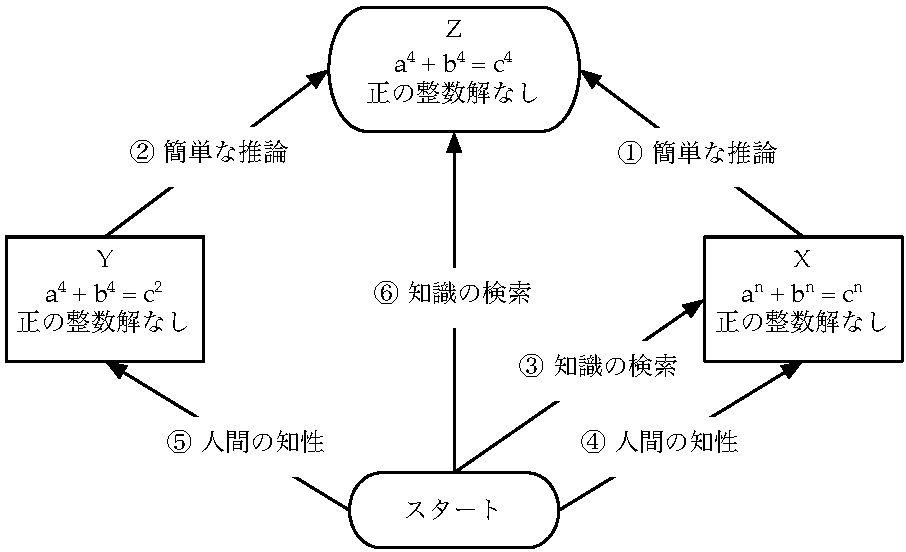
\includegraphics[width=77mm,clip]{figure.pdf}%図の幅は最大約77mm.
\caption{図の下にキャプションを丁寧に書く.(図は本文とは無関係)}\label{サンプル図}
\end{figure}

\subsubsection{表}

表\ref{サンプル表}のような,表の書き方はソースを参照せよ.複雑な表は,Excel上で作成した表を\LaTeX 形式に変換するツールを(探して)使って書くといいだろう.表の参照番号については,図の場合と同様である.

\begin{table}[htb]
\centering
\caption{表の上にキャプションを丁寧に書く.(表は本文とは無関係)}\label{サンプル表}
\begin{tabular}{cc}
\hline
文字 & コードポイント \\
\hline
\UTF{005C} & U+005C\\
\UTF{00A5} & U+00A5\\
\hline
\end{tabular}
\end{table}

\subsubsection{参考文献}\label{参考文献}

参考文献は文献データファイル(この文書では\verb|biblio.bib|)に記述する.文献データファイルはテキストファイルだから,テキストエディタで編集できる.文献データの書き方は文献\cite{参考文献リストの書き方}にまとめてあるが,慣れないうちはJabRefを使ってもいいだろう.(補足:JabRefを利用するためにはJavaの実行環境が必要である.起動後に,Options, Preferences, Appearance, Set table fontでフォントを変更する必要もあるかもしれない.)

文献の種類には,雑誌論文\cite{yabuki2011}や会議録論文\cite{数式処理システムの性能評価},卒業論文\cite{kubo2014},書籍\cite{okumura2017},ウェブサイト\cite{文章チェックリスト}などがある.文献の種類によって必要な項目が異なるため,文献\cite{参考文献リストの書き方}を見て確認すること.(補足:文献番号は句読点の前に書く.)

文献データファイルに記述した文献は\verb|\cite|で参照する(具体的な記法はソースを参照).文献番号は自動的に付けられ,文書の終わりの参考文献リストも自動的に作成される.

\subsection{原稿の処理方法}\label{原稿の処理方法}

原稿の作成に必要な作業は以下の通りである.(補足:章・節・項の見出しの後で,こういう段落なしに,いきなり箇条書きを書いてはいけない.)

\begin{enumerate}
\item TeXLiveをインストールする.
\item SumatraPDFをインストールする(Adobe AcrobatやAdobe Readerはファイルをロックするから使いにくい).
\item 原稿(\verb|draft.tex|や\verb|.bib|,\verb|.pdf|など)を用意する.(ここでは,作業ディレクトリを「\verb|C:/work|」とする.)
\item コマンドプロンプトで「\verb|c:|\UTF{23CE}\verb|cd \work|\UTF{23CE}」などとして作業ディレクトリに移動する.
\item 「\verb|uplatex -shell-escape draft|」で\LaTeX 処理,「\verb|dvipdfmx draft|」でPDF作成をするのが基本.参考文献リストが変わったときは「\verb|upbibtex draft|」を1回,参照情報が変わったときは「\verb|uplatex -shell-escape draft|」を2回実行する.\verb|fast.bat|や\verb|full.bat|を使ってもよい.途中でエラーで止まったら,「\verb|q|\UTF{23CE}」やCtrl-Cで終了する.
\item \verb|draft.pdf|をSumatraPDFで開いて結果を確認する.(補足:SyncTexの設定をしておくと,SumatraPDF上で原稿をダブルクリックすることで,\verb|.tex|のそこに対応する場所をテキストエディタで開けるようになる.)
\end{enumerate}

\subsection{原稿の提出}

原稿提出についての注意事項は以下のとおりである.

\begin{itemize}
\item 提出前に文献\cite{文章チェックリスト}を確認する.
\item 原稿を構成するファイル(\verb|.tex|や\verb|.bib|,\verb|.pdf|)を確認する.不要なファイルを提出物に含めてはいけない.
\item 原稿をGitHubのyabukilab/mainにPull Requestする.
\end{itemize}

原稿に問題がなければ,Pull Requestがマージされる.

\section{結果}

結果を書く.

\section{考察}

考察を書く.(補足:ここには主観的なことを書いてもよい.他の節はできるだけ客観的に書く.)

\section{結論}

結論を書く.(補足:ここで新しい話題を出してはいけない.)

\bibliographystyle{junsrt}
\bibliography{biblio}%「biblio.bib」というファイルが必要.

\end{document}
